\documentclass{article}
\usepackage[english,russian]{babel}
\usepackage{textcomp}
\usepackage{geometry}
  \geometry{left=2cm}
  \geometry{right=1.5cm}
  \geometry{top=1.5cm}
  \geometry{bottom=2cm}
\usepackage{tikz}
\usepackage{multicol}
\usepackage{hyperref}
\usepackage{listings}
\pagenumbering{gobble}

\lstdefinestyle{csMiptCppStyle}{
  language=C++,
  basicstyle=\linespread{1.1}\ttfamily,
  columns=fixed,
  fontadjust=true,
  basewidth=0.5em,
  keywordstyle=\color{blue}\bfseries,
  commentstyle=\color{gray},
  texcl=true,
  stringstyle=\ttfamily\color{orange!50!black},
  showstringspaces=false,
  numbersep=5pt,
  numberstyle=\tiny\color{black},
  numberfirstline=true,
  stepnumber=1,      
  numbersep=10pt,
  backgroundcolor=\color{white},
  showstringspaces=false,
  captionpos=b,
  breaklines=true
  breakatwhitespace=true,
  xleftmargin=.2in,
  extendedchars=\true,
  keepspaces = true,
  tabsize=4,
  upquote=true,
}


\lstdefinestyle{csMiptCppLinesStyle}{
  style=csMiptCppStyle,
  frame=lines,
}

\lstdefinestyle{csMiptCppBorderStyle}{
  style=csMiptCppStyle,
  framexleftmargin=5mm, 
  frame=shadowbox, 
  rulesepcolor=\color{gray}
}

\lstset{style=csMiptCppLinesStyle}
\lstset{literate={~}{{\raisebox{0.5ex}{\texttildelow}}}{1}}


\renewcommand{\thesection}{\arabic{section}}
\makeatletter
\def\@seccntformat#1{\@ifundefined{#1@cntformat}%
   {\csname the#1\endcsname\quad}%    default
   {\csname #1@cntformat\endcsname}}% enable individual control
\newcommand\section@cntformat{Часть \thesection:\space}
\makeatother



\begin{document}
\title{Семинар \#1: Библиотека SFML.\vspace{-5ex}}\date{}\maketitle


\section{Подключение библиотеки SFML}
Библиотека SFML (Simple and Fast Multimedia Library) - простая и быстрая библиотека для работы с мультимедиа. Кроссплатформенная (т. е. одна программа будет работать на операционных системах Linux, Windows и MacOS). Позволяет создавать окно, рисовать в 2D, проигрывать музыку и передавать информацию по сети. 

\subsection*{Подключение библиотеки на Windows с использованием пакетного менеджера MSYS2}
Самый простой способ установки библиотеки на компьютер -- это использованием пакетного менеджера. В данном руководстве будет рассматриваться установка библиотеки с помощью пакетного менеджера \texttt{pacman} среды MSYS2. Для того, чтобы установить SFML в среде MSYS2 проделайте следующее:
\begin{enumerate}
\item Найдите как называется пакет SFML в среде MSYS2. Для этого просто загуглите \texttt{msys2 install sfml} и одной из первых ссылок должен быть страница библиотеки SFML сайта \texttt{packages.msys2.org}. Зайдите на эту страницу и найдите команду для установки SFML. Скопируйте эту команду. Это может быть команда:
\begin{verbatim}
    pacman -S mingw-w64-x86_64-sfml
\end{verbatim}
или просто
\begin{verbatim}
    pacman -S sfml
\end{verbatim}
\item Откройте терминал MSYS2 для установки пакетов. Если у вас установлен MSYS2, то это можно сделать, нажав Пуск и начав печатать "MSYS2". 
\begin{center}
\includegraphics[scale=0.9]{../images/msys2_start.jpg}
\end{center}

\item Вставьте команду для установки SFML в терминал и нажмите Enter. 
\begin{center}
\includegraphics[scale=0.9]{../images/msys2_console.jpg}
\end{center}
Возможно потребуется нажать клавишу \texttt{Y} и Enter, чтобы подтвердить установку. После этого библиотека установится на компьютер. 

\item Убедитесь, что библиотека установилась. Для этого перейдите в папку, где установлен MSYS2, по умолчанию это \texttt{C:\textbackslash msys64}. После этого найдите папку в которой установилась библиотека SFML. Если вы используете 64-х битную версию компилятора MinGW, то библиотека установится в папке \texttt{C:\textbackslash msys64\textbackslash mingw64}. В папке \texttt{C:\textbackslash msys64\textbackslash mingw64\textbackslash bin} должны лежать \texttt{.dll} файлы библиотеки SFML. А в папке \\ \texttt{C:\textbackslash msys64\textbackslash mingw64\textbackslash include} -- заголовочные файлы библиотеки.

\item Убедитесь, что путь до папки, в которой лежат \texttt{.dll} файлы библиотеки SFML прописан в переменной среды \texttt{PATH}. Если этого пути в переменной \texttt{PATH} нет, то добавьте его.

\item Если терминал был открыт, то закройте его, а потом откройте заново.
\end{enumerate}
Всё, библиотека установлена. Теперь можно компилировать файл исходного кода, использующий библиотеку SFML следующим образом:
\begin{verbatim}
    g++ main.cpp -lsfml-graphics -lsfml-window -lsfml-system
\end{verbatim}



\subsection*{Подключение библиотеки на Linux с использованием пакетного менеджера}
Нужно установить SFML с помощью стандартного пакетного менеджера. Предположим, что используется пакетный менеджер \texttt{apt}:
\begin{verbatim}
    sudo apt install libsfml-dev
\end{verbatim}
Всё, библиотека установлена. Теперь  можно компилировать файл исходного кода, использующий библиотеку SFML следующим образом:
\begin{verbatim}
    g++ main.cpp -lsfml-graphics -lsfml-window -lsfml-system
\end{verbatim}



\subsection*{Тестирование библиотеки SFML}
Чтобы протестировать, что библиотека установилась корректно, создайте в любой директории файл \texttt{main.cpp} и поместите туда простейшую программу, использующую SFML:
\begin{lstlisting}
#include <SFML/Graphics.hpp>

int main()
{
    sf::RenderWindow window(sf::VideoMode(200, 200), "SFML works!");
    sf::CircleShape shape(100.f);
    shape.setFillColor(sf::Color::Green);

    while (window.isOpen())
    {
        sf::Event event;
        while (window.pollEvent(event))
        {
            if (event.type == sf::Event::Closed)
                window.close();
        }

        window.clear();
        window.draw(shape);
        window.display();
    }
}
\end{lstlisting}
Эту программу можно найти по адресу \href{https://www.sfml-dev.org/tutorials/2.6/start-cb.php}{https://www.sfml-dev.org/tutorials/2.6/start-cb.php}.\\
После этого зайдите в терминал, перейдите в папку, содержащую этот файл и скомпилируйте его командой:
\begin{verbatim}
    g++ main.cpp -lsfml-graphics -lsfml-window -lsfml-system
\end{verbatim}
Если SFML был установлен корректно, то программа должна скомпилироваться и в папке должен создаться исполняемый файл \texttt{a.exe} (или \texttt{a.out} на Linux). Запустите этот файл командой:
\begin{verbatim}
    .\a.exe
\end{verbatim}
или, если вы работаете на Linux, то командой:
\begin{verbatim}
    ./a.out
\end{verbatim}
Если SFML был установлен корректно, то программа должна запуститься, создать окошко размером 200 на 200 пикселей, в котором будет нарисован зелёный круг. Если это произошло, то библиотека SFML подключилась корректно.

\begin{center}
\includegraphics[scale=0.5]{../images/sfml_works.png}
\end{center}


\subsection*{Подключение вручную на Windows}
Если вы по какой-то причине не хотите использовать пакетные менеджеры (например, хотите установить другую версию библиотеки), то можно библиотеку подключить вручную. Для подключения библиотеки вам нужно сделать следующее:

\begin{enumerate}
\item Скачать нужную версию с сайта: \href{https://www.sfml-dev.org/}{sfml-dev.org}. Зайдите на этот сайт, нажмите на Downloads, а затем на Latest stable version, и выберите версию библиотеки, соответствующую вашему компилятору. Убедитесь, что версия полностью соответствует вашему компилятору, иначе библиотека не будет работать. В нашем курсе предполагается, что вы используете компилятор GCC MinGW 64-bit, но, возможно, вы используете другой компилятор.

\item Распакуйте скачанный архив. Он будет содержать папку с названием вида \texttt{SFML-<номер версии>}, например \texttt{SFML-2.6.1}. Переместите эту папку в удобное вам место на диске. Очень важно, чтобы путь до этой папки не содержал пробелы, кириллицу и какие-либо странные символы.

\item Зайдите в папку \texttt{SFML-<номер версии>}. В ней должны содержаться папки \texttt{bin}, \texttt{include}, \texttt{lib} и другие. Зайдите в папку \texttt{bin}, там должны лежать \texttt{.dll} файлы библиотеки SFML. Запомните название этой папки.

\item Добавьте в переменную среды \texttt{PATH} путь до папки, содержащей \texttt{.dll} файлы библиотеки SFML.

\item Если терминал был открыт, то закройте его, а потом откройте заново.
\end{enumerate}
Всё, библиотека установлена. Теперь можно компилировать файл исходного кода, использующий библиотеку SFML следующим образом:
\begin{verbatim}
  g++ main.cpp -I<путь до include> -L<путь до lib> -lsfml-graphics -lsfml-window -lsfml-system
\end{verbatim}
Например, если я переместил папку SFML просто на диск C и путь до этой папки это \texttt{C:\textbackslash SFML-2.6.1}, то нужная команда для компиляции будет:
\begin{verbatim}
  g++ main.cpp -I C:\SFML-2.6.1\include -L C:\SFML-2.6.1\lib -lsfml-graphics -lsfml-window -lsfml-system
\end{verbatim}
Это команда очень длинная, но вы можете вызвать её один раз. После этого можно нажимать клавишу вверх на клавиатуре, чтобы повторить команду. Или же можно просто где-то сохранить команду (в \texttt{.txt} файле на диске), а потом просто копировать её и вставлять в терминал.

\subsection*{Подключение вручную на Linux}
Этот способ совпадает со способом Windows, за исключением того, что вам не нужно устанавливать значение переменной \texttt{PATH}. Компилирование также совпадает:
\begin{verbatim}
  g++ main.cpp -I<путь до include> -L<путь до lib> -lsfml-graphics -lsfml-window -lsfml-system
\end{verbatim}

\subsection*{Использование \texttt{bat}-скрипта на Windows} 
Так как постоянно прописывать в терминале команду для компиляции может быть затруднительно, то можно положить весь процесс сборки в специальный \texttt{bat}-скрипт. \texttt{bat}-скрипт - это просто файл кода языка терминала Windows. Для того, чтобы использовать такой в файл в нашем случае нужно сделать следующее:
\begin{enumerate}
\item Cоздать в той папке, где лежит файл \texttt{main.cpp}, новый текстовый файл. 

\item Откройте этот новый текстовый файл и добавьте туда следующее:
\begin{verbatim}
  g++ %1 -I<путь до include> -L<путь до lib> -lsfml-graphics -lsfml-window -lsfml-system
  .\a.exe
\end{verbatim}
где вместо \texttt{<путь до include>} нужно подставить путь до \texttt{include} папки SFML, а вместо \texttt{<путь до lib>} -- путь до \texttt{lib} папки SFML. Сохраните и закройте файл.

\item Переименуйте этот текстовый файл в файл с расширением \texttt{.bat}. Например, в \texttt{run.bat}. Убедитесь, что ваша операционная система показывает расширения всех файлов и что файл действительно называется \texttt{run.bat}, а не, например, \texttt{run.bat.txt}.

\item Откройте терминал и в терминале зайдите в папку, содержащую файлы \texttt{main.cpp} и \texttt{run.bat}

\item Выполните в терминале команду
\begin{verbatim}
    run main.cpp
\end{verbatim}
или, если эта команда не сработала, то:
\begin{verbatim}
   .\run.bat main.cpp
\end{verbatim}
После этого всё содержимое файла \texttt{run.bat} исполнится (за место \texttt{\%1} подставится \texttt{main.cpp}), что означает, что ваша программа скомпилируется и запустится. То есть, теперь для компиляции и запуска программы достаточно написать в терминале одну команду \texttt{run}. Если понадобиться скомпилировать другую программу, то файл \texttt{run.bat} можно будет скопировать к этой программе.
\end{enumerate}

\iffalse
\subsection*{Использование \texttt{bash}-скрипта на Linux} 
Так как постоянно прописывать в терминале сборку проекта может быть затруднительно, то можно положить весь процесс сборки в специальный \texttt{bash}-скрипт. \texttt{bash}-скрипт - это просто файл кода языка терминала linux. Пример можно посмотреть в \texttt{2sfml/1bash\_script}.



\newpage
\subsection*{Подключение с помощью \texttt{cmake} (файл CMakeLists.txt)}
Система автоматической сборки \texttt{cmake} позволяет собирать большие проекты. Чтобы работать с ней вам нужно её скачать по адресу \href{https://cmake.org/}{cmake.org} и установить переменную среды \texttt{PATH}. Затем нужно создать файл \texttt{CMakeLists.txt} в директории вашего проекта и написать в нём:
\begin{verbatim}
cmake_minimum_required(VERSION 2.8.0)
project(simple_sfml)
 
# Создадим исполняемый файл по имени simple_sfml из исходного файла main.cpp
add_executable(simple_sfml main.cpp)

# Найдём библиотеку SFML автоматически с компонентами graphics, system и window
find_package(SFML 2.5 COMPONENTS graphics system window)
# Подключим эту библиотеку
target_link_libraries(simple_sfml sfml-graphics sfml-system sfml-window)
\end{verbatim}

После этого, проект можно собрать так:
\begin{verbatim}
cmake -G<генератор> <путь до CMakeLists.txt>
\end{verbatim}

Пример make-файла можно посмотреть в папке \texttt{classroom\_tasks/2sfml/4cmake} и\\ \texttt{classroom\_tasks/2sfml/5cmake\_find\_package}\\
\begin{itemize}
\item Соберите проект в папке \texttt{0basics}, используя один из приведённых выше способов (предпочтительно - make или cmake). 
\end{itemize}


\newpage
\subsection*{Работа с библиотекой:}
Документация и туториалы по библиотеке SFML можно найти на оффициальном сайте:\\ \texttt{https://www.sfml-dev.org/}{sfml-dev.org}. Пример простой программы, для работы с SFML в папке \texttt{1sfml\_basics}. \\
Основные классы SFML и их методы:
\begin{itemize}
\item[--] \texttt{sf::Vector3f, sf::Vector2f, sf::Vector2i} и т. д. Классы для математического вектора с перегруженными операциями. (аналогичные тем, что мы писали на предыдущих занятиях). \\
\href{https://www.sfml-dev.org/documentation/2.5.1/classsf_1_1Vector2.php}{sfml-dev.org/documentation/2.5.1/classsf\_1\_1Vector2.php}
\item[--] \texttt{sf::RenderWindow} - класс для окна.
\href{https://www.sfml-dev.org/documentation/2.5.1/classsf_1_1RenderWindow.php}{sfml-dev.org/documentation/2.5.1/classsf\_1\_1RenderWindow.php}
\item[--] \texttt{sf::CircleShape} - класс для фигуры - круг.
\href{https://www.sfml-dev.org/documentation/2.5.1/classsf_1_1CircleShape.php}{sfml-dev.org/documentation/2.5.1/classsf\_1\_1CircleShape.php}
\end{itemize}
\fi


\newpage
\section{Основные классы библиотеки SFML}

\subsection*{Классы математических векторов}
Классы двумерных математических векторов \texttt{sf::Vector2<T>}. У них есть два публичных поля: \texttt{x} и \texttt{y}. Также, для них перегруженны операции сложения с такими же векторами и умножения на числа. Также введены \texttt{typedef}-синонимы вроде \texttt{sf::Vector2f} для \texttt{sf::Vector2<float>}, \texttt{sf::Vector2i} для \texttt{sf::Vector2<int>}.
\begin{lstlisting}
sf::Vector2f a {1.0, 2.0};
sf::Vector2f b {3.0, -1.0};

sf::Vector2f c = 2.0f * (a + b);
std::cout << c.x << " " << c.y << std::endl;  // Напечатает  8 2
\end{lstlisting}
Но нужно помнить, что операции умножения и деления на число перегружены только с числами соответствующих типов. Например, для \texttt{sf::Vector2f} есть перегрузки только с числами типа \texttt{float}, но нет с числами типа \texttt{double} и \texttt{int}.
\begin{lstlisting}
sf::Vector2f a {1.0, 2.0};
sf::Vector2f b = 2.0f * a;  // ОК
sf::Vector2f c = 2.0 * a;   // Ошибка, нет перегрузки с числом типа double
sf::Vector2f d = 2 * a;     // Ошибка, нет перегрузки с числом типа int
\end{lstlisting}

\subsection*{Класс цвета}
Класс цвета \texttt{sf::Color}. Имеет 4 публичных поля: \texttt{r}, \texttt{g}, \texttt{b}, \texttt{a} - компоненты цвета в цветовой модели RGB и прозрачность. Есть конструктор от 3-х или 4-х аргументов. Есть перегруженные операции для сравнения и сложения цветов. Есть уже определённые цвета вроде \texttt{sf::Color::Black}, \texttt{sf::Color::Blue} и другие.

\begin{lstlisting}
sf::Color a {100, 200, 50};
sf::Color b {100, 100, 0};

sf::Color c = a + b;
std::cout << c.r << " " << c.g << " " << c.b << std::endl;  // Напечатает 200 255 50
\end{lstlisting}




\subsection*{Класс окна}
Прежде чем начать рисовать, нужно создать окно, которое будет отображать то, что мы нарисовали. Для этого в SFML есть класс \texttt{sf::RenderWindow}. Вот его основные методы:
\begin{itemize}
\item \texttt{RenderWindow(sf::VideoMode m, const sf::String\& title, sf::Uint32 style, sf::ContextSettings\& s)}
Конструктрор, с двумя обязательными и двумя необязательными аргументами. Его аргументы:
\begin{itemize}
\item Видеорежим \texttt{sf::VideoMode m} - определяет размер окна.
\item Заголовок окна \texttt{title}
\item Стиль окна \texttt{style}, необязательный аргумент, может принимать следующие значения:
\begin{itemize}
\item[-] \texttt{sf::Style::None}
\item[-] \texttt{sf::Style::Titlebar} -- окно с заголовком
\item[-] \texttt{sf::Style::Resize}  -- окно у которого можно менять размер
\item[-] \texttt{sf::Style::Close} -- окно с кнопочкой закрывания
\item[-] \texttt{sf::Style::Fullscreen} -- полноэкранный режим
\item[-] \texttt{sf::Style::Default = sf::Titlebar | sf::Resize | sf::Close} 
\end{itemize}
Этот параметр имеет значение по умолчанию (\texttt{sf::Default}).

\item Дополнительные настройки контекста OpenGL \texttt{sf::ContextSettings}, задаёт некоторые настройки окна, такие как анитиалиасинг.
\end{itemize}

\item \texttt{getPosition} и \texttt{setPosition} -- получить или установить положение окна.
\item \texttt{getSize} и \texttt{setSize} -- получить или установить размер окна в пикселях.
\item \texttt{setFramerateLimit} -- установить лимит для количества кадров в секунду.
\item \texttt{clear} -- принимает цвет и очищает скрытый холст этим цветом
\item \texttt{draw} -- рисует объект на скрытый холст
\item \texttt{display} -- отображает на экран всё что было нарисовано на скрытом холсте
\item \texttt{hasFocus} -- проверяет, активно ли окно.
\end{itemize}

\subsection*{Простая программа, которая создаёт окно зелёного цвета}
\begin{lstlisting}
#include <SFML/Graphics.hpp>
int main()
{
    sf::RenderWindow window(sf::VideoMode(800, 800), "Green Screen", sf::Style::Default);

    while (window.isOpen())
    {
        sf::Event event;
        while (window.pollEvent(event)) 
        {
            if (event.type == sf::Event::Closed)
                window.close();
        }
        window.clear(sf::Color(0, 255, 0));
        window.display();
    }
}
\end{lstlisting}

\subsection*{Классы фигур}
В SFML есть несколько классов для работы с простыми фигурами: \texttt{sf::CircleShape} (круг),\\ \texttt{sf::RectangleShape} (прямоугольник), \texttt{sf::ConvexShape} (фигура сложной формы, задаваемая точками). У этих классов есть общие методы:
\begin{itemize}
\item \texttt{setOrigin} - установить локальное начало координат фигуры. Положение этой точки задаётся относительно верхнего левого угла прямоугольника, ограничивающего фигуру. По умолчанию эта точка равна \texttt{(0, 0)}, то есть локальным началом координат фигуры считается её верхний левый угол.  Эта точка важна, так как относительно неё происходят все операции поворота и масштабирования.
\item \texttt{setPosition}, \texttt{getPosition} - задать и получить координаты фигуры. Фигура перемещается таким образом, чтобы её \texttt{origin} оказался в заданой точке.
\item \texttt{move} - принимает 2D вектор и передвигает фигуру на этот вектор.
\item \texttt{setRotation}, \texttt{getRotation} - задать и получить угол (в градусах) вращения фигуры вокруг точки \texttt{origin}
\item \texttt{rotate} - принимает вещественное число и вращает фигуру на этот угол (в градусах)
\item \texttt{setScale}, \texttt{getScale} - задать и получить величину масштабирования (2D вектор)
\item \texttt{scale} - принимает  2D вектор и растягивает или сжимает фигуру по x и по y соответственно
\item \texttt{setFillColor}, \texttt{getFillColor} -- устанавливает/возвращает цвет заливки фигуры
\end{itemize}


\subsection*{Простая программа, которая рисует движущийся круг}
\begin{lstlisting}
#include <SFML/Graphics.hpp>
int main()
{
    sf::RenderWindow window(sf::VideoMode(800, 800), "Moving Circle", sf::Style::Default);
    window.setFramerateLimit(60);
    
    sf::CircleShape circle(30);
    circle.setPosition(sf::Vector2f(100, 100));

    while (window.isOpen())
    {
        sf::Event event;
        while (window.pollEvent(event)) 
        {
            if (event.type == sf::Event::Closed)
                window.close();
        }
        circle.move(sf::Vector2f{1, 1});

        window.clear(sf::Color::Black);
        window.draw(circle);

        window.display();
    }
}
\end{lstlisting}
Пояснения по программе:

\begin{itemize}
\item В строке:
\begin{lstlisting}[frame=none]
sf::RenderWindow window(sf::VideoMode(800, 800), "Moving Circle", sf::Style::Default);
\end{lstlisting}
создаётся объект класса окна, устанавливается разрешение окна и названия окна, а также стиль окна.
\item В строке:
\begin{lstlisting}[frame=none]
window.setFramerateLimit(60);
\end{lstlisting}
Ограничивает максимальное количество кадров в секунду (англ. \textit{frames per second} или \textit{fps}) числом 60. Если не прописать эту строку, то на мощных компьютерах все движения в программе будут происходить быстрее, так как за секунду будет вполняться намного больше, чем 60 итерации главного цикла. Метод \texttt{setFramerateLimit} заставляет программу ожидать после каждого цикла, чтобы общее время одной итерации главного цикла была равна как минимум $1/60$ секунды.

Но нужно понимать, что этот метод ограничивает только максимальное количество fps. Если за один кадр выполняется много вычислений, то fps может просесть ниже 60. Из за этого все движения объектов в программе будет происходить медленнее. Чтобы скорость движения объектов не зависила от мощности компютера нужно высчитывать время, занятое на каждом кадре, и передвигать объект в соответствии с этим временем.


\item В строках:
\begin{lstlisting}[frame=none]
sf::CircleShape circle(30);
circle.setPosition(sf::Vector2f{100, 100});
\end{lstlisting}
создаём объект круга радиуса \texttt{30} и устанавливаем его положение в точку с координатами \texttt{(100, 100)}. Учтите, что в SFML ось Y направлена сверху вних. То есть значение \texttt{y = 0} будет находится в самом верху экрана, а значение \texttt{y = 800} будет находиться в самом низу нашего экрана высотой 800 пикселей.


\item Дальше, со строки:
\begin{lstlisting}[frame=none]
while (window.isOpen())
\end{lstlisting}
начинается  \textit{главный цикл} программы. Каждая итерация этого цикла -- это один кадр прогаммы. Цикл заканчивается когда у объекта окна вызовется метод \texttt{close}.

\item В строках:
\begin{lstlisting}[frame=none]
sf::Event event;
while (window.pollEvent(event)) 
{
    if (event.type == sf::Event::Closed)
        window.close();
}
\end{lstlisting}
написан \textit{цикл обработки событий}. Событиями могут быть, например, нажатие клавиш или кнопок мыши, движение мыши, изменение размера экрана, закрытие окна. За время одного кадра может произойти несколько событий. Все эти события помещаются в специальную очередь. В начале каждой итерации главного цикла нужно взять из этой очереди все события и обработать их.

В данном простом цикле обработки событий, обрабатывается только событие закрытия окна (например, нажатие на красный крестик). При нажатии на красный крестик, программа будет закрываться.

\item В строке:
\begin{lstlisting}[frame=none]
circle.move(sf::Vector2f{1, 1});
\end{lstlisting}
мы передвигаем кружок на один вправо по оси X и на один вниз по оси Y.

\item В строке:
\begin{lstlisting}[frame=none]
window.clear(sf::Color::Black);
\end{lstlisting}
мы закрашиваем \textit{скрытый холст} черным цветом. Это нужно делать, чтобы закрасить то, что было нарисовано на предыдущем кадре. Скрытый холст -- это просто двумерный массив из цветов пикселей размера \texttt{ширина окна $\times$ высота окна}, находящийся в памяти компьютера. После закраски скрытого холста никаких изменений на экране не произойдёт, так как скрытый холст на экран не отображается. В это время на экран отображается содержимое \textit{первичного холста}.


\item В строке:
\begin{lstlisting}[frame=none]
window.draw(circle);
\end{lstlisting}
кружок рисуется на скрытый холст. Опять, никаких видимых изменений на экране не будет, так как на экран отображается первичный холст.

\item В строке:
\begin{lstlisting}[frame=none]
window.display();
\end{lstlisting}
скрытый и первичный холст меняются местами. Скрытый холст становится первичным, а первичный скрытым. Теперь всё, что мы нарисовали на скрытый холст станет видимым. Такой способ чередования холстов называется \textit{двойная буферизация}. Он обеспечивает плавность анимации и отсутствие мерцаний. Если бы двойной буферизации не было, то в какие-то моменты времени мы видели бы на экране частично отрисованное изображение кадра, а в какие-то моменты весь кадр. Это выглядело бы как мерцание всех рисуемых объектов.
\end{itemize}


\newpage
\subsection*{Anti-Aliasing}
\begin{multicols}{2}
\begin{center}
\includegraphics[scale=0.5]{../images/anti-aliasing.png}
\end{center}
Вы могли заметить, что фигуры выглядят не очень красиво - имеют зазубрены. Это связано с тем, что рисования происходит на прямоугольной сетке пикселей и при проведении линий под углом образуются ступеньки. Для борьбы с этим эффектом был придуман специальный метод сглаживания, который называется антиалиасинг. Он уже автоматически реализован во всех библиотеках компьютерной графики. Чтобы установить его в SFML, нужно прописать опцию:
\begin{lstlisting}
sf::ContextSettings settings;
settings.antialiasingLevel = 8;
\end{lstlisting}
И передать \texttt{settings} на вход для конструктора \texttt{RenderWindow} четвёртым параметром. Пример в папке \texttt{code/0sfml\_basics}.
\end{multicols}


\subsection*{Класс времени}
Класс \texttt{sf::Time} для работы со временем. Есть методы \texttt{asSeconds}, \texttt{asMilliseconds} и \texttt{asMicroseconds}, которые возвращают время в виде числа в соответствующих единицах. Перегружены операторы сложения, умножения и другие. Есть дружественные функции \texttt{sf::seconds}, \texttt{sf::milliseconds} и \texttt{sf::microseconds}, которые принимают число, и возвращают соответствующие объект класса \texttt{sf::Time}. Функция \texttt{sf::sleep(sf::Time t)} -- ожидает время \texttt{t}.

\begin{lstlisting}
sf::Time t = sf::seconds(5);
sf::sleep(t);  // Программа будет ожидать 5 секунд
\end{lstlisting}

\subsection*{Класс часов}
\texttt{sf::Clock} -- это маленький класс для измерения времени. У него есть:
\begin{itemize}
\item Конструктор по умолчанию, часы запускаются автоматически после создания.
\item Метод \texttt{getElapsedTime()} -- возвращает объект \texttt{sf::Time} -- время прошедшее с последнего запуска часов.
\item Метод \texttt{restart()} -- заново запускает часы и возвращает объект \texttt{sf::Time} -- время прошедшее с предыдущего запуска часов.
\end{itemize}

\begin{lstlisting}
sf::Clock clock;

sf::Time t1 = clock.restart();
sf::sleep(sf::seconds(2));
sf::Time t2 = clock.restart();
    
std::cout << (t2 - t1).asMilliseconds() << std::endl;  // Напечатает 2000
\end{lstlisting}


\newpage



\subsection*{Класс прямоугольника}
Класс прямоугольника \texttt{sf::Rect<T>} описывает прямоугольник со сторонами параллельными осям координат.
Тип \texttt{T} задаёт тип в которых будут хранится числа, описывающие прямоугольник. Есть \texttt{typedef}-ы: \texttt{sf::FloatRect} для \texttt{sf::Rect<float>} и \texttt{sf::IntRect} для \texttt{sf::Rect<int>}.
У этого класса есть следующие публичные поля:
\begin{itemize}
\item \texttt{left} -- x-координата левой стороны прямоугольника 
\item \texttt{top} -- y-координата верхней стороны прямоугольника 
\item \texttt{width} -- ширина прямоугольника
\item \texttt{height} -- высота прямоугольника
\end{itemize}

Также у класса есть следующие методы:
\begin{itemize}
\item \texttt{bool contains(T x, T y)} -- проверяет, находится ли точка с координатами \texttt{(x, y)} внутри прямоугольника или нет.
\item \texttt{bool contains(sf::Vector2<T> p)}  -- проверяет, находится ли точка \texttt{p} внутри прямоугольника или нет.
\item \texttt{bool intersects(const sf::Rect<T>\& rect)} -- проверяет пересекается ли прямоугольник с прямоугольником \texttt{rect}.
\end{itemize}

Не следует путать класс \texttt{sf::Rect<T>} и класс фигуры \texttt{sf::RectangleShape}.
Класс \texttt{sf::Rect<T>} описывает просто прямоугольник со сторонами параллельными осям координат, с ним нельзя почти ничего делать. Класс \texttt{sf::RectangleShape} описывает прямоугольную фигуру, объекты такого класса можно перемещать, вращать, масштабировать, рисовать на экран, изменять цвет и так далее.

У фигур есть метод \texttt{getGlobalBounds}, который возвращает прямоугольник со сторонами параллельными осям координат, описанный вокруг фигуры.
\begin{lstlisting}
sf::CircleShape c(50);
sf::FloatRect r = c.getGlobalBounds();  // Прямоугольник r описанный вокруг фигуры круга c

// Проверим, находится ли точка p внутри прямоугольника r
sf::Vector2f p {30, 30};
if (r.contains(p))
    std::cout << "Point inside Rect!" << std::endl;
\end{lstlisting}

\subsection*{Класс строки}
В SFML есть свой класс строки под названием \texttt{sf::String}. Поддерживает разные виды кодировок. Имеет конструкторы от стандартных строк \texttt{C++} и строк в стиле \texttt{C}. Для работы с кириллицей эту строку нужно инициализировать широким строковым литералом. В отличии от обычного он предваряется буквой \texttt{L}.
\begin{lstlisting}
sf::String a = "Hello";
sf::String b = L"Привет";
\end{lstlisting}

\subsection*{Класс шрифта}
Класс шрифта \texttt{sf::Font} нужен для загрузки данных шрифта с диска и использования этого шрифта при отрисовке текста. Файл шрифта можно найти в интернете, он имеет расширение \texttt{.ttf}. Загрузить шрифт в программу можно с помощью метода \texttt{loadFromFile} класса \texttt{sf::Font}:
\begin{lstlisting}
sf::Font font;
if (!font.loadFromFile("consola.ttf")) 
{
    std::cout << "Error. Can't load font!" << std::endl;
    std::exit(1);
}
\end{lstlisting}
Метод \texttt{loadFromFile} будет искать файл относительно исполняемого файла. То есть в примере выше нужно убедиться, что файл \texttt{consola.ttf} лежит в той же папке, что и исполняемый файл.

\subsection*{Класс текста}
\texttt{sf::Text} -- класс объекта для отображения текста на экране.
У объектов этого класса можно задать шрифт, содержимое строки, размер шрифта, цвет, стиль с помощью соответствующих методов. Положение текста на экране задаётся с помощью методов, аналогичных методам фигур: \texttt{setPosition}, \texttt{move}, \texttt{rotate} и других.

\subsection*{Пример программы, которая рисует вращающийся текст}
\begin{lstlisting}
#include <SFML/Graphics.hpp>
#include <iostream>
int main()
{
    sf::RenderWindow window(sf::VideoMode(800, 800), "Rotating Text", sf::Style::Default);
    window.setFramerateLimit(60);
    
    sf::Font font;
    if (!font.loadFromFile("consola.ttf")) 
    {
        std::cout << "Error! Can't load font!" << std::endl;
        std::exit(1);
    }

    sf::Text text;
    text.setFont(font);
    text.setString(L"Привет");
    text.setCharacterSize(50);
    text.setFillColor(sf::Color(70, 160, 100));
    text.setStyle(sf::Text::Bold | sf::Text::Underlined);
    text.setPosition({300, 200});

    while (window.isOpen())
    {
        sf::Event event;
        while (window.pollEvent(event)) 
        {
            if (event.type == sf::Event::Closed)
                window.close();
        }
        text.rotate(0.1f);

        window.clear(sf::Color::Black);
        window.draw(text);

        window.display();
    }
}
\end{lstlisting}

\newpage
\subsection*{Опасность при использовании \texttt{sf::Font} и \texttt{sf::Text}}
При работе с классами \texttt{sf::Font} и \texttt{sf::Text} нужно понимать, что \texttt{sf::Text} хранит внутри себя не весь шрифт, а только указатель на шрифт. То есть, при задании шрифта у текста:
\begin{lstlisting}[frame=none]
text.setFont(font);
\end{lstlisting}
в объект \texttt{sf::Text} НЕ копируется весь объект \texttt{sf::Font}, а копируется только адресс объекта \texttt{sf::Font}.\\
Следовательно, если соответствующий объект шрифта уничтожится раньше объекта текста, то в объекте текста будет храниться висячая ссылка на шрифт и работа с таким текстом приведёт к неопределённому поведению.

\begin{lstlisting}
#include <iostream>
#include <SFML/Graphics.hpp>

sf::Text getText(std::string fontFile)
{
    sf::Font font;
    if (!font.loadFromFile(fontFile))
    {
        std::cout << "Error! Can't load font!" << std::endl;
        std::exit(1);
    }
    sf::Text text;
    text.setFont(font);
    text.setString(L"Привет");
    text.setCharacterSize(50);
    text.setFillColor(sf::Color(70, 160, 100));
    text.setStyle(sf::Text::Bold | sf::Text::Underlined);
    text.setPosition({300, 200});
    return text;
}

int main()
{
    sf::RenderWindow window(sf::VideoMode(800, 800), "Rotating Text", sf::Style::Default);
    window.setFramerateLimit(60);
    
    // Создаём текст, но объект sf::Font создастся и уничтожится внутри функции getText
    sf::Text text = getText("consola.ttf");
    // Далее объект text хранит в себе указатель на удалённый объект sf::Font
    while (window.isOpen())
    {
        sf::Event event;
        while (window.pollEvent(event)) 
        {
            if (event.type == sf::Event::Closed)
                window.close();
        }
        text.rotate(0.1f);
        window.clear(sf::Color::Black);
        window.draw(text);  // UB
        window.display();
    }
}
\end{lstlisting}

\newpage
\subsection*{Рисование прямых линий}
Под линией в программировании понимается не линия в математическом смысле этого слова, а прямой отрезок, ограниченный двумя точками.

Рисование прямых линий в коде не похоже на рисование фигур. В библиотеке нет специального класса, описывающего отдельную линию, но есть класс \texttt{sf::Vertex} описывающий вершину, имеющую некоторые координаты и цвет.
Для того, чтобы нарисовать линии нужно сначала создать массив, хранящий вершины этих линий. Для рисования одной линии нужен массив из двух вершин, но можно отрисовать сразу много линий, если создать массив из большого количества вершин.
После того, как массив создан, нужно вызвать перегрузку метода \texttt{draw} класса \texttt{sf::RenderWindow}, которая предназначена для рисования линий. У этой перегрузки есть 3 параметра:

\begin{itemize}
\item Массив вершин
\item Количество вершин для отрисовки
\item Тип примитива отрисовки. Может принимать следующие значения:
\begin{itemize}
\item \texttt{sf::Lines} рисует не соединённые линии.
Если в массиве $n$ вершин, то нарисует $n / 2$ линий.
\item \texttt{sf::LineStrip} рисует соединённые линии. 
Если в массиве $n$ вершин, то нарисует $n - 1$ линий.
\item Есть ещё несколько примитивов, но мы их использовать не будем.
\end{itemize}
\end{itemize}

Пример программы, которая рисует 2 белых линии: линию с координатами \texttt{\{(0, 0), (50, 100)\}} и линию с координатами \texttt{\{(200, 200), (400, 400)\}}.
\begin{lstlisting}
#include <SFML/Graphics.hpp>
int main()
{
    sf::RenderWindow window(sf::VideoMode(800, 800), "Drawing Lines", sf::Style::Default);
    
    sf::Vertex vertices[] =
    {
        sf::Vertex(sf::Vector2f(0, 0),     sf::Color::White),
        sf::Vertex(sf::Vector2f(50, 100),  sf::Color::White),
        sf::Vertex(sf::Vector2f(200, 200), sf::Color::White),
        sf::Vertex(sf::Vector2f(400, 400), sf::Color::White)
    };
    
    while (window.isOpen())
    {
        sf::Event event;
        while (window.pollEvent(event)) 
        {
            if (event.type == sf::Event::Closed)
                window.close();
        }
        window.clear(sf::Color::Black);
        
        window.draw(vertices, 4, sf::Lines);
        // window.draw(vertices, 4, sf::LineStrip);
        
        window.display();
    }
}
\end{lstlisting}
Если в качестве типа примитива выбрать \texttt{sf::LineStrip}, то дополнительно нарисуется линия с координатами \texttt{\{(50, 100), (200, 200)\}}.


\subsection*{Рисование кривых}
SFML не поддерживает рисование кривых линий напрямую. Для того, чтобы нарисовать кривую, нужно нарисовать её, используя большое количество маленьких прямых линий.
Например, код ниже рисует синусоиду:
\begin{lstlisting}
#include <cmath>
#include <SFML/Graphics.hpp>
int main()
{
    sf::RenderWindow window(sf::VideoMode(800, 800), "Drawing Sin Func", sf::Style::Default);
    
    std::vector<sf::Vertex> vertices;
    for (int i = 0; i < 200; ++i)
    {
        float x = 4 * i;
        float y = 400 + 100 * std::sin(x / 30);
        vertices.push_back(sf::Vertex(sf::Vector2f(x, y), sf::Color::White));
    }
    
    while (window.isOpen())
    {
        sf::Event event;
        while (window.pollEvent(event)) 
        {
            if (event.type == sf::Event::Closed)
                window.close();
        }
        window.clear(sf::Color::Black);
        window.draw(vertices.data(), vertices.size(), sf::LineStrip);
        window.display();
    }
}
\end{lstlisting}


\subsection*{Рисование линий с толщиной}
Предыдущий способ рисования линий рисует линии с толщиной в 1 пиксель. SFML не поддерживает рисование линий, толщиной в несколько пикселей напрямую. Есть два способа отрисовки линии с толщиной:
\begin{itemize}
\item Использовать тип примитива \texttt{sf::TriangleStrip} при отрисовке линий. Но при этом нужно добавить дополнительные вершины в массив.
\item Вместо линий можно рисовать очень тонкие прямоугольники, например как это сделано в этой функции:
\end{itemize} 
\begin{lstlisting}
void drawThickLine(sf::RenderWindow& window, sf::Vector2f start, sf::Vector2f finish, float thickness, sf::Color c)
{
    static sf::RectangleShape rect;
    sf::Vector2f r = finish - start;
    rect.setSize({std::sqrt(r.x * r.x + r.y * r.y), thickness});
    rect.setFillColor(c);
    rect.setOrigin({0, thickness / 2});
    rect.setPosition(start);
    rect.setRotation(std::atan2(r.y, r.x) * 180 / std::numbers::pi);
    window.draw(rect);
}
\end{lstlisting}


\subsection*{Класс клавиатуры}
Класс клавиатуры \texttt{sf::Keyboard} используется для проверки нажата ли та или иная клавиша в данный момент. Для проверки используется статический метод этого класса \texttt{isKeyPressed}. Этому методу нужно передать на вход код клавиши. Код клавиши можно получить, также используя класс \texttt{sf::Keyboard}. 

Внутри класса \texttt{sf::Keyboard} находится \texttt{enum}, который описывает все эти коды. Примеры кодов клавиш:
\begin{verbatim}
Space, Enter, Escape, LShift, RShift, LControl, Left, Right, Up, Down, W, A, S, D ...
\end{verbatim}
То есть, например, для клавиши пробел нужно использовать 
\texttt{sf::Keyboard::Space}.

\subsection*{Программа, рисующая круг, который движется только тогда, когда зажата клавиша Пробел (Space)}
\begin{lstlisting}
#include <SFML/Graphics.hpp>
int main()
{
    sf::RenderWindow window(sf::VideoMode(800, 800), "Moving Circle", sf::Style::Default);
    window.setFramerateLimit(60);
    sf::CircleShape circle(30);
    circle.setPosition(sf::Vector2f(100, 100));

    while (window.isOpen())
    {
        sf::Event event;
        while (window.pollEvent(event)) 
        {
            if (event.type == sf::Event::Closed)
                window.close();
        }
        
        if (sf::Keyboard::isKeyPressed(sf::Keyboard::Space))
        	circle.move(sf::Vector2f{1, 1});

        window.clear(sf::Color::Black);
        window.draw(circle);

        window.display();
    }
}
\end{lstlisting}

\subsection*{Класс мыши. Проверка на нажатие кнопок мыши.}
Класс мыши \texttt{sf::Mouse} похож на класс клавиатуры. Проверка на нажатие кнопок мыши происходит схожим образом:
\begin{lstlisting}
// Проверка на то, что нажата левая кнопка мыши
if (sf::Mouse::isButtonPressed(sf::Mouse::Left))
	...

// Проверка на то, что нажато колёсико мыши
if (sf::Mouse::isButtonPressed(sf::Mouse::Middle))
	...
\end{lstlisting}
Для того, чтобы лучше понимать как получать координаты курсора мыши, разберёмся сначала какие системы координат сущеструют в SFML.


\section{Системы координат в SFML}
В библиотеки SFML существуют несколько систем координат. Одни из частых ошибок при работе с библиотекой -- это ошибки связанные с системами координат. Если передать в функцию, которая принимает точку в одной системе, точку из другой системы координат, то поведение программы будет не таким, каким вы ожидали.

Рассмотрим следующие 2 системы координат:
\begin{enumerate}
\item Система координат сетки пикселей
\item Система координат мира объектов
\end{enumerate}
Для определённости будем предполагать, что окно имеет размеры 400 на 400 пикселей.

\subsection*{Система координат сетки пикселей.}
\begin{itemize}
\item В этой системе описывается положение каждого пикселя в окне.
\item Центр координат -- в верхнем левом углу окна. 
\item Ось $Ox$ идёт слева направо, ось $Oy$ -- сверху вниз.
\item Эта система целочисленная. Координаты хранятся в числах типа \texttt{int}. Для хранения точки обычно используется \texttt{sf::Vector2i}.
\item Нижний правый угол имеет координаты, соответствующие размерам окна (в данном случае \texttt{(400, 400)}).
\item При изменении размеров окна, размер также сетки пикселей меняется. Соответственно, при изменении размеров окна, координаты нижнего правого угла изменятся.
\item В этой системе координат обычно возращаются координаты курсора мыши функциями библиотеки.
\end{itemize}


\vspace{1cm}
\begin{center}
\includegraphics[scale=0.9]{../images/system_pixels.png}
\end{center}



\subsection*{Система координат мира объектов}
\begin{itemize}
\item В этой системе описывается положение объектов (кругов, прямоугольников, линий и т. д.).
\item Центр координат -- по умолчанию в верхнем левом углу окна. 
\item Ось $Ox$ идёт слева направо, ось $Oy$ -- сверху вниз.
\item Эта вещественная система координат. Координаты хранятся в числах типа \texttt{float}. Для хранения точки обычно используется \texttt{sf::Vector2f}.
\item Нижний правый угол имеет координаты, соответствующие размерам окна при запуске программы (в данному случае \texttt{(400.0, 400.0)}).
\item При изменении размеров окна, в окне продолжается отображаться та же самая часть мира объектов.
Соответственно, при изменении размеров окна координаты нижнего правого угла НЕ изменятся.
\item Эту систему координат можно перенастроить, используя класс \texttt{sf::View}.
\end{itemize}

\vspace{1cm}
\begin{center}
\includegraphics[scale=0.9]{../images/system_coords.png}
\end{center}





\newpage
\subsection*{Различие между системой координат пикселей и системой координат мира}
Эти две системы координат можно легко перепутать, так как при запуске программы все точки на экране имеют совпадающие значения в обоих системах координат. Разница же в системах координат проявится только если размер окна будет изменён. 

Например, предположим, что у нас было окно размером 400 на 400 пикселей, и затем мы его сжали в 2 раза по горизонтали, так что размер окна стал 200 на 400 пикселей. 
После такого преобразования сетка пикселей также стала меньше в 2 раза Отрисовываемая область мира же при этом не изменилась. В окне по-прежнему будут отображаться те же самые объект, что и до сжатия, только теперь они будут также сжаты в 2 раза.
Теперь точки в окне имеют разные значения в разных системах координат. Если вы будете использовать координаты из одной системы в той функции, где требуются координаты из другой системы, то программа будет вести себя некорректно.

\vspace{0.5cm}
\begin{minipage}{0.5\textwidth}
\begin{center}
Система координат пикселей
\includegraphics[scale=1]{../images/system_pixels_narrow.png}
\end{center}
\end{minipage}
\begin{minipage}{0.5\textwidth}
\begin{center}
Система координат мира
\includegraphics[scale=1]{../images/system_coords_narrow.png}
\end{center}
\end{minipage}
\vspace{0.5cm}


\subsection*{Конвертация координат из системы координат пикселей в систему координат мира}
Для конвертации точки из одной системы координат в другую используются методы класса \texttt{sf::RenderWindow}:
\begin{itemize}
\item \texttt{Vector2f 	mapPixelToCoords(Vector2i point)} -- конвертирует точку из системы координат пикселей в систему координат мира.
\item \texttt{Vector2i 	mapCoordsToPixel(Vector2f point)} -- конвертирует точку из системы координат мира в систему координат пикселей.
\end{itemize}
\begin{lstlisting}[frame=none]
sf::Vector2i p {200, 200};                    // Координаты пикселя (200, 200)
sf::Vector2f q = window.mapPixelToCoords(p);  // Координаты точки в мире, соответствующие 
                                              // этому пикселю
\end{lstlisting}


\newpage
\subsection*{Класс мыши. Получение координат курсора мыши.}
Помимо того, что класс мыши \texttt{sf::Mouse} позволяет проверить была ли нажата та или иная кнопка мыши, он также может может дать координаты курсора мыши. Для этой цели в классе \texttt{sf::Mouse} есть следующие статические методы:
\begin{itemize}
\item \texttt{getPosition(const sf::Window\&)} -- возвращает положение курсора мыши в координатах пикселей окна.
\item \texttt{setPosition(const sf::Vector2i\&, const sf::Window\&)} --  устанавливает положение курсора мыши в координатах пикселей окна.
\end{itemize}
Обратите внимание, что эти функции работают в системе координат пикселей. Если вы хотите использовать координаты мыши, полученные из этих функций, в функции, которая работает в системе координат мира, то нужно будет сделать преобразование координат с помощью метода \texttt{mapPixelToCoords}.


\subsection*{Пример программы, которая перемещает круг к курсору, при нажатии на ЛКМ}
\begin{lstlisting}
#include <SFML/Graphics.hpp>
int main()
{
    sf::RenderWindow window(sf::VideoMode(800, 800), "Circle and Mouse");
    window.setFramerateLimit(60);
    
    sf::CircleShape c(50);
    c.setOrigin({50, 50});
    c.setFillColor(sf::Color::Green);
    
    while (window.isOpen())
    {
        sf::Event event;
        while (window.pollEvent(event)) 
        {
            if (event.type == sf::Event::Closed)
                window.close();
        }
        
        if (sf::Mouse::isButtonPressed(sf::Mouse::Left))
        {
            sf::Vector2i mousePixel = sf::Mouse::getPosition(window);
            sf::Vector2f mousePosition = window.mapPixelToCoords(mousePixel);
            c.setPosition(mousePosition);
        }
        window.clear(sf::Color::Black);
        window.draw(c);
        window.display();
    }
}
\end{lstlisting}
Попробуйте самостоятельно ответить на следующие вопросы:
\begin{itemize}
\item Что делает метод \texttt{setOrigin} класса \texttt{sf::CircleShape}? Почему в этот метод передаются именно такие значения? Что будет если убрать строку с вызовом этого метода или передать другие значения?
\item Что если не делать преобразование координат \texttt{mapPixelToCoords}, а просто сразу передать координаты пикселя в метод \texttt{setPosition} как это сделано в строках ниже? Будет ли программа работать корректно?
\begin{lstlisting}[frame=none]
sf::Vector2i mousePixel = sf::Mouse::getPosition(window);
c.setPosition({(float)mousePixel.x, (float)mousePixel.y});
\end{lstlisting}
\end{itemize}


\newpage
\section{Примеры программ с использованием библиотеки SFML}
Рассмотрим примеры программ, рисующих движущиеся шарики в 2-х измерениях.  Больше примеров можно найти в папках \texttt{code/1ball\_movement} и \texttt{code/2many\_balls}.

\subsection*{Зацикленное движение шарика в 2d пространстве}
Программа рисует один шарик, двигающийся с постоянной скоростью, но если шарик выходит за границы окна, он появляется с другой стороны.

Для того, чтобы добиться такого поведения шарика, мы будем просто проверять координаты шарика каждый кадр, и если, например, x-координата шарика будет больше ширины экрана, то мы просто будем вычитать из x-координата шарика значение ширины экрана. Более точно, нужно учесть ещё радиус шарика и перемещать его только тогда, когда он полностью выходит за границы окна.

\begin{lstlisting}
#include <SFML/Graphics.hpp>

int main()
{
    sf::RenderWindow window(sf::VideoMode(800, 800), "Moving Ball Cycle", sf::Style::Default);
    window.setFramerateLimit(60);
    
    // Создаём шарик радиуса 30 в точке с координатами (100, 100)
    sf::CircleShape ball(30);
    ball.setOrigin(sf::Vector2f{ball.getRadius(), ball.getRadius()});
    ball.setPosition(sf::Vector2f{100, 100});

    while (window.isOpen())
    {
        sf::Event event;
        while (window.pollEvent(event)) 
        {
            if (event.type == sf::Event::Closed)
                window.close();
        }
        
        // Передвигаем шарик на вектор (10, 5)
        ball.move(sf::Vector2f{10, 5});
	
		// Если шарик выходит за границы окна, он появляется с другой стороны:
        sf::Vector2f max = window.getView().getSize(); // размеры окна
        if (ball.getPosition().x - ball.getRadius() > max.x)
            ball.move({-max.x - 2 * ball.getRadius(), 0});
        if (ball.getPosition().y - ball.getRadius() > max.y)
            ball.move({0, -max.y - 2 * ball.getRadius()});

        window.clear(sf::Color::Black);
        window.draw(ball);

        window.display();
    }
}
\end{lstlisting}


\subsection*{Движение шарика в гравитационном поле с упругими столкновениями от границ}
\begin{lstlisting}
#include <SFML/Graphics.hpp>
int main()
{
    sf::RenderWindow window(sf::VideoMode(800, 800), "Collisions and Gravity");
    window.setFramerateLimit(60);
 
 	// Создаём шарик радиуса 30 в точке (100, 100)
    sf::CircleShape ball(30);
    ball.setOrigin({ball.getRadius(), ball.getRadius()});
    ball.setPosition(sf::Vector2f{100, 100});

	// Задаём начальную скорость и ускорение шарика
    sf::Vector2f ballVelocity {300, 0};
    sf::Vector2f ballAcceleration {0, 1000};
    float dt = 1.0f / 60;

    while (window.isOpen())
    {
        sf::Event event;
        while (window.pollEvent(event)) 
        {
            if (event.type == sf::Event::Closed)
                window.close();
        }
        
        // Уравнения движения
        ballVelocity += ballAcceleration * dt;
        ball.move(ballVelocity * dt);
		
        sf::Vector2f max = window.getView().getSize(); // размеры окна
        
        // Обрабатываем столкновения со стенками:
        if (ball.getPosition().x + ball.getRadius() > max.x)
            ballVelocity.x *= -1;
            
        if (ball.getPosition().x - ball.getRadius() < 0)
            ballVelocity.x *= -1;
            
        if (ball.getPosition().y + ball.getRadius() > max.y)
            ballVelocity.y *= -1;
            
        if (ball.getPosition().y - ball.getRadius() < 0)
            ballVelocity.y *= -1;

        window.clear(sf::Color::Black);
        window.draw(ball);
        window.display();
    }
}
\end{lstlisting}

\subsection*{Работа с несколькими шариками}
Для создания программы, которая рисует множество шариков, удобно написать класс, отвечающий за управление движением каждого отдельного шарика.
\begin{lstlisting}
class Ball
{
private:
    sf::RenderWindow& mRenderWindow;
    sf::Vector2f mPosition {};
    sf::Vector2f mVelocity {};
    float mRadius          {};
public:
    Ball(sf::RenderWindow& window) : mRenderWindow{window} {}

    void update(float dt)
    {
        mPosition += mVelocity * dt;
        handleCollisions();
    }

    void handleCollisions()
    {
        sf::Vector2f max = mRenderWindow.getView().getSize();
        if (float dx = mPosition.x + mRadius - max.x; dx > 0)
            mVelocity.x *= -1;
            
        if (float dx = -mPosition.x + mRadius; dx > 0)
            mVelocity.x *= -1;

        if (float dy = mPosition.y + mRadius - max.y; dy > 0)
            mVelocity.y *= -1;

        if (float dy = -mPosition.y + mRadius; dy > 0)
            mVelocity.y *= -1;
    }

    void draw() const
    {
        static sf::CircleShape circle;
        circle.setFillColor(sf::Color::White);
        circle.setRadius(mRadius);
        circle.setOrigin({mRadius, mRadius});
        circle.setPosition(mPosition);
        mRenderWindow.draw(circle);
    }
    void setPosition(sf::Vector2f position) {mPosition = position;}
    void setVelocity(sf::Vector2f velocity) {mVelocity = velocity;}
    void setRadius(float radius)            {mRadius = radius;}
    sf::Vector2f getPosition() const {return mPosition;}
    sf::Vector2f getVelocity() const {return mVelocity;}
    float        getRadius()   const {return mRadius;}
};
\end{lstlisting}
После этого создадим контейнер (например, \texttt{std::vector}) и будем хранить в нём необходимое число шариков:
\begin{lstlisting}
sf::RenderWindow window(sf::VideoMode(800, 800), "Many Balls + Collisions");
window.setFramerateLimit(60);
float dt = 1.0f / 60;

std::vector<Ball> balls;
for (int i = 0; i < 10; ++i)
{
    Ball ball{window};
    ball.setRadius(10);
    ball.setPosition({200.0f + 50.0f * i, 600.0f - 50.0f * i});             
    ball.setVelocity({500, 500});
    balls.push_back(ball);
}
\end{lstlisting}
Для передвижения шариков, обработки столкновений со стенками и отрисовки, просто пробегаем по контейнеру и вызываем соответствующий метод шарика:
\begin{lstlisting}

while (window.isOpen())
{
    sf::Event event;
    while (window.pollEvent(event)) 
    {
        if (event.type == sf::Event::Closed)
            window.close();
    }

    for (auto& ball : balls)
        ball.update(dt);
    
    window.clear(sf::Color::Black);   
    for (auto& ball : balls)
        ball.draw();
    window.display();
}
\end{lstlisting}


\newpage

\section{События}
События (англ. \textit{events}) -- это механизм обработки пользовательского ввода и других действий, происходящих в окне приложения. События могут включать в себя нажатия клавиш, движение мыши, закрытие окна и т. д. \\
Класс \texttt{sf::Event} используется для хранения информации о произошедшем событии. Объекты этого класса содержат тип события и дополнительные данные, связанные с ним (например, какая клавиша была нажата или координаты курсора мыши).

Рассмотрим пример программы, использующей события. Следующая программа рисует круг и передвигает его при каждом нажатии на клавишу пробел (\texttt{sf::Keyboard::Space}):
\begin{lstlisting}
#include <SFML/Graphics.hpp>
int main()
{
    sf::RenderWindow window(sf::VideoMode(800, 800), "Key Pressed Event");
    window.setFramerateLimit(60);

    sf::CircleShape circle(50);
    circle.setOrigin({circle.getRadius(), circle.getRadius()});
    circle.setPosition({100, 400});

    while (window.isOpen())  // Главный цикл
    {
        sf::Event event;
        while (window.pollEvent(event))  // Цикл обработки событий
        {
            if (event.type == sf::Event::Closed)
                window.close();
                
            if (event.type == sf::Event::KeyPressed)
            {
                if (event.key.code == sf::Keyboard::Space)
                    circle.move({50, 0});
            }
        }

        window.clear(sf::Color::Black);
        window.draw(circle);
        window.display();
    }
}
\end{lstlisting}
Пояснения по программе:
\begin{itemize}
\item Сначала мы создаём объект типа \texttt{sf::Event}, который может хранить внутри себя информацию о событии.

\item Метод \texttt{pollEvent} принимает объект \texttt{event} по ссылке, затем извлекает одно событие из внутренней \textit{очереди событий} и присваивает объекту \texttt{event} это событие. Метод \texttt{pollEvent} возвращает \texttt{true}, если в очереди событий было хотя бы одно событие, и \texttt{false}, если очередь событий была пуста. Таким образом цикл обработки событий работает до тех пор пока в очереди событий не закончатся события.

\item Очередь событий -- это специальная очередь внутри SFML, которая хранит в себе все события, произошедшие за время текущего кадра. В начале каждого кадра мы извлекаем поочерёдно все события из этой очереди и обрабатываем их.

\item После того как событие из очереди получено, его нужно обработать. Будем обрабатывать по-разному в зависимости от типа события. Тип события хранится в поле \texttt{event.type}.
\end{itemize}


\newpage
\subsection*{Типы событий в библиотеке SFML}
\begin{itemize}
\item \texttt{sf::Event::Closed} -- событие, которое происходит когда пользователь пытается закрыть окно, например, когда нажимает на красный крестик в углу окна или когда использует комбинацию клавиш \texttt{Alt + F4}.

\item \texttt{sf::Event::KeyPressed} -- происходит когда пользователь нажал на какую либо клавишу. Код клавиши хранится в поле \texttt{event.key.code}.

\item \texttt{sf::Event::KeyReleased} -- происходит когда пользователь отпустил какую либо клавишу. Код клавиши также хранится в поле \texttt{event.key.code}.

\item \texttt{sf::Event::MouseButtonPressed} -- происходит когда пользователь нажал на какую либо кнопку мыши. Код кнопки мыши хранится в поле \texttt{event.mouseButton.button}. Координаты мыши в момент нажатия в системе координат пикселей хранятся в полях \texttt{event.mouseButton.x} и \texttt{event.mouseButton.y}.

\item \texttt{sf::Event::MouseButtonReleased} -- происходит когда пользователь отпустил какую либо кнопку мыши. Код кнопки мыши хранится в поле \texttt{event.mouseButton.button}. Координаты мыши в момент отпускания в системе координат пикселей хранятся в полях \texttt{event.mouseButton.x} и \texttt{event.mouseButton.y}.

\item \texttt{sf::Event::MouseMoved} -- происходит когда пользователь передвинул курсор мыши. Координаты мыши в момент передвижения курсора в системе координат пикселей хранятся в полях \texttt{event.mouseMove.x} и \texttt{event.mouseMove.y}. Обратите внимание, что название поля в котором хранятся координаты мыши отличается для этого события.

\item \texttt{sf::Event::MouseWheelScrolled} -- происходит когда пользователь прокручивает колёсико мыши.
\end{itemize}

\subsection*{Очередь событий}
Очередь событий (англ. \textit{event queue}) -- это очередь, хранящая объекты событий (\texttt{std::queue<sf::Event>}) и находящаяся внутри библиотеки SFML. Напрямуя с этой очередь мы взаимодействовать не можем. События добавляются в эту очередь автоматически при нажатии на клавиши, кнопкок и т. д.. События извлекаются из очереди с помощью метода \texttt{pollEvent}.
\begin{center}
\includegraphics[scale=0.9]{../images/event_queue.png}
\end{center}
В начале каждого кадра из очереди извлекаются и обрабатываются все накопленные события. Это означает, что в любой момент времени в очереди находятся только те события, которые произошли в течение текущего кадра



\newpage
\subsection*{Пример обработки событий. События нажатия и отпускания кнопки мыши}
Данная программа, обрабатывает нажатия и отпускания левой клавиши мыши (ЛКМ).
Программа рисует белый круг.
При нажатии на ЛКМ круг меняет свой цвет на красный.
При отпускании ЛКМ круг опять становится белым.
\begin{lstlisting}
#include <SFML/Graphics.hpp>

int main()
{
    sf::RenderWindow window(sf::VideoMode(800, 800), "Mouse Button Pressed or Relesed");
    window.setFramerateLimit(60);
    
    sf::CircleShape circle(200);
    circle.setPosition({200, 200});

    while (window.isOpen()) 
    {
        sf::Event event;
        while (window.pollEvent(event)) 
        {
            if (event.type == sf::Event::Closed)
                window.close();

            if (event.type == sf::Event::MouseButtonPressed)
            {
                if (event.mouseButton.button == sf::Mouse::Left)
                    circle.setFillColor(sf::Color::Red);
            }

            if (event.type == sf::Event::MouseButtonReleased)
            {
                if (event.mouseButton.button == sf::Mouse::Left)
                    circle.setFillColor(sf::Color::White);
            }
        }

        window.clear(sf::Color::Black);
        window.draw(circle);
        window.display();
    }
}
\end{lstlisting}



\newpage
\subsection*{Пример обработки событий. Получение координат мыши при нажатии.}
Координаты мыши для событий \texttt{MouseButtonPressed} и \texttt{MouseButtonReleased} хранятся в полях \texttt{event.mouseButton.x} и \texttt{event.mouseButton.y}. Однако это координаты в системе координат пикселей. Для того, чтобы перевести эти координаты в систему координат мира нужно использовать метод \texttt{mapPixelToCoords}. Если этого не сделать, то программа будет работать некорректно, при изменении размеров окна.

Следующая программа рисует кружок. При нажатии на левую кнопку мыши кружок меняет положение на то, в котором находится курсор. Также, при нажатии, программа печатает в консоль координаты мыши в системе координат пикселей и в системе координат мира.
\begin{lstlisting}
#include <SFML/Graphics.hpp>
#include <iostream>

int main()
{
    sf::RenderWindow window(sf::VideoMode(800, 600), "Mouse Button Pressed Coordinates");
    window.setFramerateLimit(60);

    sf::CircleShape circle(30);
    circle.setOrigin({circle.getRadius(), circle.getRadius()});
    circle.setPosition({200, 200});

    while (window.isOpen()) 
    {
        sf::Event event;
        while (window.pollEvent(event)) 
        {
            if (event.type == sf::Event::Closed)
                window.close();

            if (event.type == sf::Event::MouseButtonPressed)
            {
                if (event.mouseButton.button == sf::Mouse::Left)
                {
                    sf::Vector2i mousePixel {event.mouseButton.x, event.mouseButton.y};
                    sf::Vector2f mousePosition = window.mapPixelToCoords(mousePixel);

                    std::cout << "Left Mouse Button is pressed\n";
                    std::cout << "Pixel: " << mousePixel.x << " " << mousePixel.y;
                    std::cout << std::endl;
                    std::cout << "Position: " << mousePosition.x << " " << mousePosition.y;
                    std::cout << std::endl;

                    circle.setPosition(mousePosition);
                }
            }
        }

        window.clear(sf::Color::Black);
        window.draw(circle);
        window.display();
    }
}
\end{lstlisting}

\newpage
\subsection*{Пример обработки событий. Получение координат мыши при перемещении курсора.}

Следующая программа рисует кружок, который перемещается вслед за курсором. Для этого обрабатывается событие \texttt{sf::Event::MouseMoved}. Координаты мыши в этом событии хранятся в полях \texttt{event.mouseMove.x} и \texttt{event.mouseMove.у}. 

\textbf{Обратите внимание, что названия полей в котором хранятся координаты мыши для этого события отличается от событий нажатия и отпускания кнопки мыши!}. Если использовать поля\\ \texttt{event.mouseButton.x} и \texttt{event.mouseButton.у} вместо полей \texttt{event.mouseMove.x} и \texttt{event.mouseMove.у} при обработке этого события, это приведёт к некорректной работе программы.
\begin{lstlisting}
#include <SFML/Graphics.hpp>
int main()
{
    sf::RenderWindow window(sf::VideoMode(800, 800), "Mouse Button Move Coordinates");
    window.setFramerateLimit(60);

    sf::CircleShape circle(30);
    circle.setOrigin({circle.getRadius(), circle.getRadius()});
    circle.setPosition({400, 400});

    while (window.isOpen()) 
    {
        sf::Event event;
        while (window.pollEvent(event)) 
        {
            if (event.type == sf::Event::Closed)
                window.close();

            if (event.type == sf::Event::MouseMoved)
            {
                sf::Vector2i mousePixel {event.mouseMove.x, event.mouseMove.y};
                sf::Vector2f mousePosition = window.mapPixelToCoords(mousePixel);
                circle.setPosition(mousePosition);
            }
        }
        window.clear(sf::Color::Black);
        window.draw(circle);
        window.display();
    }
}
\end{lstlisting}

Эти и другие примеры работы с событиями в SFML можно найти в папке \texttt{code/4events}.


\newpage
\subsection*{Различие между двумя видами обработки нажатий клавиш и кнопок}
Как вы могли заметить, в библиотеке SFML есть два способа обработки нажатий на клавиши и кнопки:
\begin{enumerate}
\item Проверка, нажата ли та или иная клавиша в данный момент, с помощью статических методов классов \texttt{sf::Keyboard} и \texttt{sf::Mouse}.
\item Использование механизма событий.
\end{enumerate}
Два этих способа различаются друг от друга. Разберём отличия на примере нажатия левой кнопки мыши:
\subsubsection*{Проверка нажатия на ЛКМ с использованием метода класса \texttt{sf::Mouse}}
\begin{minipage}{0.64\textwidth}
\begin{lstlisting}[frame=none]
while (window.isOpen()) 
{
    sf::Event event;
    while (window.pollEvent(event)) 
    {
        if (event.type == sf::Event::Closed)
            window.close();
    }
	
	if (sf::Mouse::isButtonPressed(sf::Mouse::Left))  
		std::cout << "LMB is pressed" << std::endl; 
    
    window.clear(sf::Color::Black);
    window.display();
}
\end{lstlisting}
\end{minipage}
\begin{minipage}{0.36\textwidth}
\begin{itemize}
\item Проверяет, зажата ли ЛКМ в данный момент.
\item Действие, соответствующее зажатию клавиши будет происходить каждый кадр во время которого была зажата ЛКМ.
\item Если вы нажали ЛКМ, а затем отпустили через 10 кадров, то действие произойдёт 10 раз.
\item Если вы нажали и отпустили ЛКМ вне проверки (это может произойти если программа "подвисла"), то действие не произойдёт ни разу.
\item Лучше использовать, если нужно проверить, что кнопка \texttt{зажата}.
\end{itemize}
\end{minipage}

\subsubsection*{Проверка нажатия на ЛКМ с использованием событий}
\begin{minipage}{0.64\textwidth}
\begin{lstlisting}[frame=none]
while (window.isOpen()) 
{
    sf::Event event;
    while (window.pollEvent(event)) 
    {
        if (event.type == sf::Event::Closed)
            window.close();

        if (event.type == sf::Event::MouseButtonPressed)
        {
            if (event.mouseButton.button == sf::Mouse::Left)
                std::cout << "LMB is pressed" << std::endl; 
        }
    }

    window.clear(sf::Color::Black);
    window.display();
}
\end{lstlisting}
\end{minipage}
\begin{minipage}{0.36\textwidth}
\begin{itemize}
\item Проверяет, была ли нажата ЛКМ с момента предыдущего цикла обработки событий.
\item Действие, соответствующее нажатию клавиши произойдёт ровно 1 раз за каждое нажатие.
\item Если вы нажали ЛКМ, а затем отпустили через 10 кадров, то действие произойдёт 1 раз.
\item Если вы нажали и отпустили ЛКМ вне проверки (это может произойти если программа "подвисла"), то действие тоже произойдёт 1 раз.
\item Лучше использовать, если нужно отловить нажатие кнопки. Под нажатием понимается момент перехода из состояния \texttt{кнопка не зажата} в состояние \texttt{кнопка зажата}.
\end{itemize}
\end{minipage}

\newpage
Предположим, что программа работает с частотой 100 кадров в секунду.
Далее, предположим, что вы нажали на кнопку мыши и держали её зажатой 5 секунд, а потом отпустили.
Тогда процесс нажатия, зажатия и отпускания кнопки мыши можно проиллюстрировать на следующей схеме:
\\

\begin{center}
\includegraphics[scale=1]{../images/mouse_presses.png}
\end{center}


\subsection*{Автоповтор при нажатиях на клавиши клавиатуры}
События, возникающие при нажатии клавиш клавиатуры, несколько отличаются от событий, связанных с нажатием кнопок мыши. Чтобы наглядно продемонстрировать это различие, рассмотрим конкретный пример. Представьте, что вы открыли текстовый редактор и зажали клавишу \texttt{A} на некоторое время. Что произойдёт? Будет ли добавлен только один символ \texttt{A}, или новые символы будут появляться непрерывно? На самом деле, процесс будет следующим:
\begin{itemize}
\item Первый символ \texttt{A} добавиться сразу при нажатии.
\item Второй символ \texttt{A} добавиться через некоторое относительно долгое время.
\item Все последующие символы \texttt{A} будут добавляться с очень короткой задержкой между ними.
\end{itemize}

Такое поведение при зажатиях клавиш наблюдается не только в текстовых редекторах, но и в большинстве других приложений. Это связано с тем, что данная функциональность реализована на уровне операционной системы. Она была добавлена для того, чтобы сделать взаимодействие с клавиатурой более удобным и предсказуемым.
Таким образом, с точки зрения операционной системы, событие, соответствующее нажатию клавиши, происходит не только в момент её физического нажатия, но и в определённые моменты при её удержании. Это позволяет системе генерировать повторяющиеся события, которые обрабатываются приложениями для реализации автоповтора.

Вводятся следующие определения:
\begin{itemize}
\item Задержка повтора (англ. \textit{Repeat Delay}) -- время между моментом нажатия клавиши и началом автоповтора событий, связанных с этой клавишей, при её удержании.
Значение этого параметра равно около \textit{500 мс}.
\item Частота повторений (англ. \textit{Repeat Rate}) -- частота, с которым события  повторяются после начала автоповтора при удержании клавиши.
Обычно, значение этого параметра равно примерно \textit{1 / (40 мс)}.
Обратите внимание, что даже при автоповторе события обычно повторяются реже чем кадры.
\end{itemize}

Процесс нажатия, зажатия и отпускания клавиши клавиатуры можно проиллюстрировать на схеме:

\begin{center}
\includegraphics[scale=1]{../images/keyboard_presses.png}
\end{center}

В библиотеке SFML событие \texttt{sf::Event::KeyPressed} происходит не только при непосредственном нажатии на клавишу, но и при автоповторе.


\newpage
\section{Реализация элементов графического интерфейса}
Графический интерфейс пользователя (англ. \textit{Graphical User Interface} или \textit{GUI}) — это способ взаимодействия пользователя с программой или устройством, основанный на визуальных элементах, таких как кнопки, меню, окна, иконки и другие графические компоненты. В данной части попробуем реализовать некоторые простые элементы графического интерфейса, используя библиотеку SFML.
Больще примеров реализаций можно найти в папке \texttt{code/5gui}.

\subsection*{Перетаскиваемая табличка}
Перетаскиваемая табличка (англ. \textit{draggable}) -- простейший элемент графического интерфейса. Представляет собой прямоугольник, который можно перетаскивать, используя  мышь.
\subsubsection*{Реализация перетаскиваемой таблички без использования класса}
 Для реализации такого элемента интерфейса заведём следующие переменные:
\begin{list}{$\circ$}{}  
\item \texttt{draggableShape} -- прямоугольник, то есть объект типа \texttt{sf::RectangleShape}, используемый для хранения положения и цвета прямоугольника, а также для его отрисовки.
\item \texttt{isDragged} -- булевое значение, которое равно \texttt{true}, в те моменты, когда табличка перетаскивается.
\item \texttt{offset} -- двумерный вектор, равный разницей между положением курсора мыши и положением верхнего левого угла таблички в момент последнего нажатия на табличку.
\end{list}
Будем делать следующее:
\begin{itemize}
\item При событии нажатия на левую кнопку мыши:
\begin{itemize}
\item Проверять, находился ли курсор мыши внутри прямоугольника в момент нажатия.\\
Если да, то делаем следующие два шага.
\item Устанавливаем значение переменной \texttt{isDragged = true}.
\item Устанавливаем значение переменной \texttt{offset = mousePosition - draggableShape.getPosition()}
\end{itemize}

\item При событии движения курсора мыши:
\begin{itemize}
\item Если \texttt{isDragged} находится в состоянии \texttt{true}, то будем устанавливаем значение положения прямоугольника как \texttt{draggableShape.setPosition(mousePosition - offset)}.
\end{itemize}

\item При событии отпускания левой кнопки мыши:
\begin{itemize}
\item Устанавливаем значение переменной \texttt{isDragged = false}.
\end{itemize}
\end{itemize}
\begin{center}
\includegraphics[scale=1]{../images/draggable.png}
\end{center}
Полный код этой реализации можно найти в папке \texttt{code/5gui/0draggable/0no\_class}.

\subsubsection*{Реализация перетаскиваемой таблички с созданием класса \texttt{Draggable}}
Гораздо удобнее создать класс (назовём его \texttt{Draggable}), который будет полностью описывать перетаскиваемые таблички. В этот класс мы поместим все необходимые переменные и функции, описывающие этот элемент интерфейса. Полный код этой реализации можно найти в папке \texttt{code/5gui/0draggable/1using\_class}.

После того, как такой класс создан, можно легко написать программу, которая использует сразу несколько таких перетаскиваемых табличек. Пример можно посмотреть в  \texttt{code/5gui/0draggable/2cards}.

\newpage
\subsection*{Кнопка}
Попробуем создать кнопку. Логика работы кнопки должна быть аналогичной логике работы обычной кнопки в ОС Windows. Требования к простейшей кнопке такие:
\begin{enumerate}
\item Кнопка представляет собой прямоугольник.
\item Изначально кнопка имеет некоторый заданный цвет.
\item При наведении курсора мыши на кнопку, её цвет меняется.
\item При нажатии и зажатии левой кнопки мыши (ЛКМ) над кнопкой, её цвет меняется на цвет, отличный от первых двух.
\item При отпускании ЛКМ, если курсор всё ещё находится на прямоугольнике, происходит некоторое действие (например, печать в консоль).
\item В иных случаях действие не происходит (например, если мы зажали ЛКМ вне кнопки и отпустили над кнопкой или если мы зажали ЛКМ над кнопкой и отпустили вне кнопки).
\end{enumerate}
Реализацию простейшей кнопки можно найти тут: \texttt{code/5gui/1button}.
Для того, чтобы реализовать кнопку, создадим класс \texttt{Button}, который будет состоять из следующих полей:
\begin{list}{$\circ$}{}  
\item \texttt{sf::RectangleShape mShape} -- объект класса прямоугольника SFML. Внутри \texttt{mShape} хранятся координаты, размеры и текущий цвет прямоугольника, предствляющего нашу кнопку.
\item \texttt{sf::Color mDefaultColor} -- цвет кнопки, когда она не зажата и на неё не наведён курсор.
\item \texttt{sf::Color mHoverColor} -- цвет кнопки, когда она не зажата, но на неё наведён курсор.
\item \texttt{sf::Color mPressedColor} -- цвет кнопки, когда она находится в зажатом состоянии.
\item \texttt{bool mIsPressed} -- переменная, равная \texttt{true}, когда кнопка находится в зажатом состоянии.
\item \texttt{sf::RenderWindow\& mRenderWindow} -- также храним ссылку на окно SFML, на которое будем отрисовывать кнопку. Эту ссылку можно было бы не хранить, а просто передавать во все функции, где окно понадобится, но тогда код был бы более громоздким.
\end{list}
Также у класса будут следующие публичные методы:
\begin{list}{$\circ$}{}  
\item \texttt{void draw()} -- рисует кнопку на окне. Ссылка на окно хранится внутри объекта \texttt{Button}. Поэтому тут её передавать не нужно.
\item \texttt{bool handleEvent(const sf::Event\& event)} -- принимает событие, и обрабатывает всё, что касается кнопки. Возвращает \texttt{true}, если кнопка была нажата за время предыдущего кадра.
\end{list}
\quad 

\begin{center}
\includegraphics[scale=0.9]{../images/button.png}
\end{center}
Для того, чтобы реализовать кнопку, делаем следующее. При событии нажатия на ЛКМ, если курсор находится внутри кнопки, то устанавливаем значение \texttt{mIsPressed = true}. При событии отпускания ЛКМ, если \texttt{mIsPressed == true} и курсор также находится внутри кнопки, то клик на кнопку произошёл, и мы устанавливаем \texttt{mIsPressed = false} и возвращаем \texttt{true} из метода \texttt{handleEvent}.


\clearpage
\subsection*{Слайдер}
Слайдер -- это элемент графического интерфейса, который позволяет пользователю выбирать значение из определённого диапазона, перемещая ползунок вдоль горизонтальной или вертикальной шкалы. Компоненты слайдера:
\begin{itemize}
\item Ползунок (англ. \textit{thumb}) -- подвижный элемент, который пользователь перетаскивает для выбора значения.
\item Шкала (англ. \textit{track}) -- линия или дорожка, вдоль которой перемещается ползунок.
\end{itemize}
\quad

\begin{center}
\includegraphics[scale=0.9]{../images/slider.png}
\end{center}
Реализацию простейшего слайдера можно найти тут: \texttt{code/5gui/2slider}.
Для того, чтобы реализовать слайдер, создадим класс \texttt{Slider}, состоящий из следующих полей:
\begin{list}{$\circ$}{}  
\item \texttt{sf::RectangleShape mTrackShape} -- объект класса прямоугольника, который представляет шкалу прокрутки. Внутри хранятся положение, размеры и цвет шкалы прокрутки.
\item \texttt{sf::RectangleShape mThumbShape} -- объект класса прямоугольника, который представляет ползунок. Внутри хранятся положение, размеры и цвет ползунка.
\item \texttt{bool mIsPressed} -- Эта переменная равна \texttt{true}, когда ползунок находится в нажатом состоянии.
\item \texttt{sf::RenderWindow\& mRenderWindow} -- также храним ссылку на окно SFML, на которое будем отрисовывать кнопку. Эту ссылку можно было бы не хранить, а просто передавать во все функции, где окно понадобится, но тогда код был бы более громоздким.
\end{list}
Также у класса будут следующие публичные методы:
\begin{list}{$\circ$}{}  
\item \texttt{void draw()} -- рисует слайдер на окне. Ссылка на окно хранится внутри объекта \texttt{Slider}. Поэтому тут её передавать не нужно.
\item \texttt{bool handleEvent(const sf::Event\& event)} -- обрабатывает всё, что касается слайдера.
\item \texttt{float getValue()} -- возращает значение положения слайдера от 0 до 100.
\end{list}
Для начала создадим вспомогательный метод, который бы устанавливал положение ползунка с учётом ограничений на его движение. Изменять положение ползунка будем только с использованием этого метода.
\begin{lstlisting}[frame=none]
void setRestrictedThumbPosition(sf::Vector2f position)
{
    float min = mTrackShape.getPosition().x - mTrackShape.getSize().x / 2.0f;
    float max = mTrackShape.getPosition().x + mTrackShape.getSize().x / 2.0f;
    mThumbShape.setPosition({std::clamp(position.x, min, max), mThumbShape.getPosition().y});
}
\end{lstlisting}
Чтобы реализовать класс слайдера делаем следующее.
\begin{itemize}
\item При событии нажатия на левую кнопку мыши:
если курсор мыши находится внути прямоугольника ползунка или внутри прямоугольника шкалы, то изменяем положение ползунка на положение курсора (используя \texttt{setRestrictedThumbPosition}) и устанавливаем \texttt{mIsPressed = true}.
\item При событии движения курсора мыши: если \texttt{mIsPressed == true}, то изменяем положение ползунка на положение курсора (используя \texttt{setRestrictedThumbPosition}).
\item При событии отпускания левой кнопки мыши: устанавливаем \texttt{mIsPressed = false}.
\end{itemize}
\iffalse
\newpage
\section{Задачи}
\begin{itemize}

\item \textbf{Шарики:} В папке \texttt{collision\_circles} содержится заготовка кода. 
\begin{itemize}
\item Используйте этот код, чтобы найти пересечение двух шаров. Если в процессе движения шары начнут накладываются друг на друга, то они должны окрашиваться в красный цвет. После прекращения наложения, шары должны опять стать белыми. Для этого добавьте поле типа \texttt{sf::Color} в класс \texttt{Ball} и метод \texttt{bool is\_colliding(const Ball\& b) const}, который будет проверять 2 кружка на столкновение.
\item Измените программу так, чтобы кружки упруго отскакивали друг от друга. Для этого нужно, при столкновении шариков, обратить составляющую скорости параллельную прямой, соединяющую центры шариков.
\item Добавьте возможность добавления нового шарика по нажатию правой кнопки мыши.
\item Добавьте возможность стенки по нажатию левой кнопки мыши. Нужно зажать ЛКМ в одной точки и отпустить в другой, чтобы получить стенку. Стенка -- это просто отрезок. Но шарики должны от него должны отскакивать. Про обнаружение столкновений можно посмотреть в папке \texttt{collision\_examples}.
\end{itemize}
\end{itemize}
\fi



\end{document}